\chapter[Love Across Branches]{Love\\Across Branches}

\vspace{1em}
\hfill
\begin{minipage}[c]{0.6\textwidth}
\raggedleft
\small\itshape
For one human being to love another: that is perhaps the most difficult of all our tasks, the work for which all other work is but preparation.\\[0.5em]
\upshape\footnotesize Rainer Maria Rilke, \textit{Letters to a Young Poet} (1929)
\end{minipage}%
\hspace{0.5em}
\begin{minipage}[c]{0.12\textwidth}
% \includegraphics[width=\textwidth]{figures/ch13_love.png}
\end{minipage}
\vspace{1.5em}

\noindent \textsc{Worldlines had an image for love.} Two worldlines, two curves through spacetime, drawing close and winding around each other, each bending the other's path. A braid in the manifold. Not a metaphor for love but the geometry of it: where two lives shape each other, the structure itself carries a braid, and the braid is as real and as permanent as anything else at its coordinates.

This book takes the image and thickens it.

\section*{The braid, frayed}

You and the person you love can each be described as changing patterns rather than perfectly bounded substances. If Everett or Picture A is true, related descriptions may include histories in which you never met, met and parted, or remained together. Figure~\ref{fig:braid} makes that conditional picture visible. The relationship here does not depend on settling it.

\begin{figure}[h]
\centering
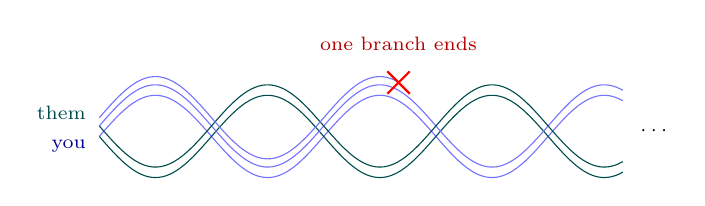
\begin{tikzpicture}[scale=0.95]
  % two many-stranded patterns weaving
  \foreach \dy in {-0.07,0.07} {
    \draw[blue!55, thin] plot[smooth, domain=0:7, samples=80] (\x, {1.2+\dy+0.55*sin(\x*120)});
    \draw[teal!60!black, thin] plot[smooth, domain=0:7, samples=80] (\x, {1.2+\dy-0.55*sin(\x*120)});
  }
  % one strand ends partway (a branch where the worldline terminates)
  \draw[blue!55, thin] plot[smooth, domain=0:4.0, samples=50] (\x, {1.38+0.55*sin(\x*120)});
  \draw[thick, red] (3.85,2.0) -- (4.15,1.7);
  \draw[thick, red] (3.85,1.7) -- (4.15,2.0);
  % labels
  \node[font=\scriptsize, blue!55!black, anchor=east] at (-0.05,1.0) {you};
  \node[font=\scriptsize, teal!60!black, anchor=east] at (-0.05,1.45) {them};
  \node[font=\scriptsize, red!70!black, anchor=south] at (4.0,2.15) {one branch ends};
  \node[font=\scriptsize, anchor=west] at (7.1,1.2) {$\cdots$};
\end{tikzpicture}
\caption{A conditional Everettian picture of the braid. If decoherent branches are ontically real, related histories may continue differently. The equal strands encode no branch count or weight, and the diagram makes no claim that continuation occurs in ``most'' branches. The local relation is whole without being totaled across them.}
\label{fig:braid}
\end{figure}

One reaction to this picture is that it cheapens the thing. If there were countless similar relations, would this one become a fraction of a total?

No. Moral importance is not divided by a hypothetical copy count. The braid here, between you and the person in the room, is not one-millionth of a braid if similar patterns are described elsewhere. Its importance arises in the lives it shapes here.

\section*{What is and is not your business}

Here the framework asks for a discipline, and it is the one that runs under the whole of Part III.

Possible other braids are not within your causal reach, whether or not Picture A is true. Moral action travels along actual connections: the person in the room, the next call, the unanswered message. You need not assert distant occurrences to refuse indifference toward possible suffering. Orientation can be broad; action remains local.

What this leaves you is small, and it is not nothing. The braid at these coordinates is what you have, and tending it is the whole of what is available. ``Enough'' here does not mean maximal, and it does not mean consoling. It means what is here, attended to. That is the only form care has ever taken, in any framework. The Library does not change what care is. It only removes the fantasy that there was ever more on offer than the coordinates you actually occupy. The braid is a cut you keep making; the structure keeps none of them for you.

\section*{Two at a table}

The abstraction has been doing a great deal of work, so set it down for a moment and look at the thing itself. A kitchen, late. The specific person across the table, holding a mug the way they always hold it, both hands, though the coffee went cold an hour ago. A conversation you have had before and may have again. None of it is underwritten. The labels \emph{you}, \emph{them}, and \emph{us} are models, but this is the table where your actions have effects tonight.

And the mug is still warm enough to hold. The sentence is still unfinished. The person holding it is this one and not an abstract class. That is a whole encounter, owing nothing to descriptions in which the chair is empty or occupied by someone else. This is the one your hands can touch.

This is what tending looks like with the metaphysics taken out: not a bond the cosmos maintains on your behalf, but two finite people in a room for a while. The acts stay concrete. You refill the mug. You finish the sentence kindly instead of sharply. You stay at the table a little past when you meant to leave. No global measure confers value on the staying; its value is in what it does to the people there.

\section*{The braid that went wrong}

The honesty cuts the other way too, and the book will not pretend otherwise.

Picture A permits cruel descriptions as readily as kind ones. That symmetry is not a moral ledger, and the framework does not establish their instantiation. The carelessness in your own past cannot be mended by imagining a kinder version elsewhere.

This is the cold the book keeps returning to. It does not offer multiplicity as a ledger in which kind possibilities cancel cruel ones. There is no cancellation. There is what happened here, and what you do next.

What you do next is the move you have, and it is worth making. You act here, with this person, for care, knowing the framework neither requires nor rewards it. The braid you tend is the one your hands are on.

\section*{Whose braid}

There is a question this chapter has leaned on without asking. The braid is between two patterns, you and another. But what is a pattern, that it can be loved, or do the loving? The word \emph{you} has been carrying a great deal, and the next chapter finally examines it. The braid, it will turn out, is between two labels, two conventions an observer draws around regions of the structure. That sounds as though it should weaken the braid further. It does the opposite, and it is the last thing the book needs in place before it can say what it has been building toward.

The next chapter takes up the self.
